\section{Entrenamiento y experimentación con modelos generativos}
El proceso de desarrollo del sistema generativo se ha abordado desde una perspectiva experimental, orientada a identificar, comparar y refinar diferentes arquitecturas capaces de transformar texto en imagen. Este capítulo recoge las principales fases de exploración realizadas, desde aproximaciones iniciales con redes generativas adversarias simples hasta la implementación final con modelos de difusión.

Durante esta etapa se han probado múltiples configuraciones, técnicas de entrenamiento y datasets, en un proceso iterativo que ha permitido evaluar los puntos fuertes y débiles de cada solución. Las pruebas realizadas han sido fundamentales no solo para mejorar la calidad de las imágenes generadas, sino también para asegurar que el sistema pudiera adaptarse a las restricciones técnicas del entorno y responder adecuadamente a las necesidades planteadas en los requisitos del proyecto.

En las siguientes secciones se describen en detalle las distintas aproximaciones evaluadas, los criterios utilizados para su comparación y las decisiones técnicas que condujeron al diseño final del sistema.


\subsection{Primera aproximación: GAN}

Como punto de partida en el desarrollo del sistema generativo, se optó por implementar una Red Generativa Adversaria (GAN) clásica. Esta elección respondió a su simplicidad conceptual y a la extensa documentación existente que la convierte en una excelente base para experimentar con modelos generativos. La implementación inicial permitió adquirir una comprensión profunda del funcionamiento adversarial entre el generador y el discriminador, y sentar las bases para una posterior transición hacia arquitecturas más avanzadas.

Las GANs tradicionales operan sin condicionamiento explícito, es decir, generan imágenes sin ningún tipo de control externo sobre el contenido. Si bien esto limita la aplicabilidad directa para sistemas de búsqueda visual guiados por texto, su valor como primera aproximación radicó en que permitieron validar el flujo de entrenamiento, optimizar el entorno de ejecución y establecer un punto de referencia inicial de calidad de las imágenes generadas.

\subsubsection{Librerías, herramientas y datasets}

Para la implementación se utilizaron \textbf{Keras} y \textbf{TensorFlow}, dos frameworks ampliamente adoptados en la comunidad de aprendizaje profundo. Keras, con su API de alto nivel, facilitó la definición de modelos de forma modular y legible, mientras que TensorFlow proporcionó soporte para operaciones eficientes en GPU y una gestión estable del grafo computacional. Esta combinación permitió iterar rápidamente en la definición y entrenamiento de las redes.

En cuanto a los datos, se seleccionaron dos conjuntos integrados en la propia librería de Keras: \textbf{CIFAR-10} y \textbf{CIFAR-100}. Ambos constan de 60.000 imágenes a color de resolución 32x32 píxeles, distribuidas equitativamente entre clases. CIFAR-10 contiene 10 categorías genéricas (como coches, animales, aviones), lo que lo convierte en un dataset óptimo para pruebas preliminares. Por su parte, CIFAR-100 agrupa las imágenes en 100 clases más específicas, lo que representa un desafío considerable mayor para la generalización del modelo generador.

\subsubsection{Pruebas y resultados}

La arquitectura definida para esta fase inicial consistió en una red generativa compuesta por varias capas convolucionales transpuestas, activadas con \texttt{ReLU}, que transformaban un vector latente aleatorio de 100 dimensiones en una imagen RGB de 32x32 píxeles. El discriminador, en contrapartida, estaba constituido por una red con capas convolucionales convencionales y activaciones \texttt{LeakyReLU}, cuya salida final indicaba la probabilidad de que una imagen fuese real o generada.

Durante el entrenamiento con CIFAR-10 se llevaron a cabo múltiples iteraciones para estudiar el comportamiento del modelo:

En una primera fase experimental, se utilizó una tasa de aprendizaje de 0.0002 junto con el optimizador \texttt{Adam}, obteniéndose imágenes que reflejaban estructuras rudimentarias, pero carecían de nitidez y riqueza de detalle. Uno de los primeros hallazgos fue que el discriminador aprendía más rápidamente que el generador, generando un desequilibrio que provocaba el estancamiento del entrenamiento.

Para mitigar este efecto, se redujo la tasa de aprendizaje a 0.0001, lo que produjo una convergencia más suave. Sin embargo, las imágenes seguían mostrando ruido y distorsiones. En una tercera iteración, se decidió aumentar la capacidad del generador, introduciendo capas adicionales e incrementando la dimensionalidad de las capas intermedias. Este ajuste permitió generar imágenes ligeramente más definidas, aunque seguían siendo poco coherentes a nivel semántico.

Con el dataset CIFAR-100, el proceso se replicó bajo condiciones similares. No obstante, el salto en complejidad del conjunto de datos se tradujo en mayores dificultades para el modelo. En las etapas iniciales, las imágenes generadas eran considerablemente más borrosas y la red mostraba dificultades para aprender patrones distinguibles. Para contrarrestar el sobreajuste del discriminador, se introdujeron capas \texttt{Dropout} y se aplicaron nuevas reducciones a la tasa de aprendizaje. Se exploraron, además, modificaciones estructurales en el generador, como la inclusión de \texttt{BatchNormalization} y ajustes en las funciones de activación, pero sin éxito significativo en la calidad final.

Los resultados más representativos de estos experimentos se sintetizan en la Tabla~\ref{tab:gan_experimentos}, donde se detallan los principales hiperparámetros, ajustes arquitectónicos realizados y observaciones obtenidas para cada fase de entrenamiento con los datasets CIFAR-10 y CIFAR-100.

\begin{table}[H]
    \centering
    \renewcommand{\arraystretch}{1.5}
    \begin{tabular}{|>{\columncolor{gray!10}}p{2.8cm}|p{3.8cm}|p{4.1cm}|p{4.1cm}|}
        \hline
        \rowcolor{gray!30}
        \textbf{Experimento} & \textbf{Hiperparámetros} & \textbf{Modificaciones} & \textbf{Resultados} \\
        \hline
        \textbf{CIFAR-10:\newline Fase 1} & LR=0.0002, Adam, 50 épocas & Arquitectura estándar de DCGAN & Imágenes básicas con baja resolución y poco detalle. \\
        \hline
        \textbf{CIFAR-10:\newline Fase 2} & LR=0.0001, Adam & Sin cambios en arquitectura & Mejor estabilidad, pero mucho ruido. \\
        \hline
        \textbf{CIFAR-10:\newline Fase 3} & LR=0.0001, más capas, mayor dimensionalidad & Generador más profundo, mayor capacidad & Ligera mejora en detalle, pero sin correspondencia clara con clases. \\
        \hline
        \textbf{CIFAR-100:\newline Fase 1} & LR=0.0002, Adam & Arquitectura igual que CIFAR-10 & Alta dificultad de convergencia. Imágenes más borrosas. \\
        \hline
        \textbf{CIFAR-100:\newline Fase 2} & LR=0.0001, Dropout en Discriminador & Regularización para evitar sobreajuste & Mejor equilibrio de pérdidas, pero sin mejora clara en calidad. \\
        \hline
        \textbf{CIFAR-100:\newline Fase 3} & LR=0.0001, arquitectura ampliada & Capas adicionales, mayor profundidad en generador & Imágenes aún con ruido y baja fidelidad semántica. \\
        \hline
    \end{tabular}
    \caption{Resumen de experimentos con GAN: configuración y resultados}
    \label{tab:gan_experimentos}
\end{table}


\subsubsection{Conclusión}

La primera aproximación mediante una GAN básica resultó útil desde una perspectiva formativa y técnica: permitió familiarizarse con los ciclos de entrenamiento, con la interacción generador-discriminador y con el entorno de ejecución completo. Además, ofreció una referencia sobre la calidad base que se puede obtener sin condicionamiento.

Sin embargo, también dejó patente que este enfoque no era suficiente para el objetivo del proyecto: generar imágenes condicionadas por descripciones textuales. La incapacidad de controlar el contenido generado y la baja calidad semántica de las salidas evidenciaron la necesidad de incorporar mecanismos de control explícito. Así, esta experiencia motivó el paso a la siguiente etapa: el uso de redes generativas adversarias condicionales, que permitirían introducir un vector de características (por ejemplo, proveniente de una descripción textual) como condición del proceso generativo.

\subsection{Condicionalidad: cGAN}
A diferencia de las tradicionales, las Redes Generativas Adversarias Condicionales (cGAN) permiten generar imágenes a partir de una condición explícita, como un vector de características derivado de una descripción textual. Esta capacidad resultaba fundamental para los objetivos del proyecto, por lo que se planteó como un enfoque prometedor desde el inicio.

\subsubsection{Librerías y Herramientas}
La implementación de la cGAN se llevó a cabo empleando herramientas ya utilizadas en la fase anterior con GAN básicas, como Keras y TensorFlow, por su robustez y facilidad de desarrollo. Además, se utilizaron NumPy y Matplotlib para el preprocesamiento de datos y la visualización de resultados, respectivamente. El dataset elegido fue COCO (Common Objects in Context), que destaca por incluir una gran variedad de imágenes, cada una acompañada por cinco descripciones textuales detalladas. Esto lo hace ideal para experimentar con modelos de generación condicionada por texto.

\subsubsection{Procesamiento de Texto}
Para representar las descripciones textuales de entrada, se probaron distintos enfoques. Inicialmente se utilizó \textit{one-hot encoding}, por su simplicidad de implementación, aunque se descartó rápidamente debido a su alta dimensionalidad y su incapacidad para capturar relaciones semánticas entre palabras.

Posteriormente, se probó Word2Vec, que transforma palabras en vectores de características en un espacio semántico. Esta técnica mejoró la representación textual, pero mostró limitaciones al no capturar adecuadamente la estructura de las frases ni las relaciones entre los objetos.

Finalmente, se optó por trabajar directamente con las descripciones originales del dataset COCO, que ya estaban preprocesadas y estructuradas. Estas descripciones fueron tokenizadas y limpiadas para eliminar ruido textual. Se utilizaron embeddings preentrenados como los de CLIP, que transforman las frases en vectores latentes significativos para la generación de imágenes. Esta solución resultó más robusta, computacionalmente eficiente y adecuada para preservar la semántica de las descripciones complejas.

\subsubsection{Pruebas preliminares con MNIST}
Antes de abordar un dataset complejo como COCO, se realizó una prueba de concepto utilizando el conjunto de datos MNIST. Este dataset contiene imágenes de dígitos del 0 al 9, por lo que era ideal para comprobar la capacidad de la cGAN para generar imágenes condicionadas.

Se codificaron los dígitos como vectores one-hot y se concatenaron con el ruido aleatorio que se proporciona al generador. El modelo se entrenó durante 50 épocas con una tasa de aprendizaje de 0.0002 y un tamaño de batch de 64. Al principio, las imágenes eran borrosas, pero al finalizar el entrenamiento, la cGAN era capaz de generar dígitos nítidos y variados, respetando la condición de entrada. Este comportamiento puede observarse en la Figura \ref{fig:numeros_0-9}, que muestra los dígitos generados al final del proceso. Esto confirmó la viabilidad del enfoque condicional.

\begin{figure}[H]
\centering
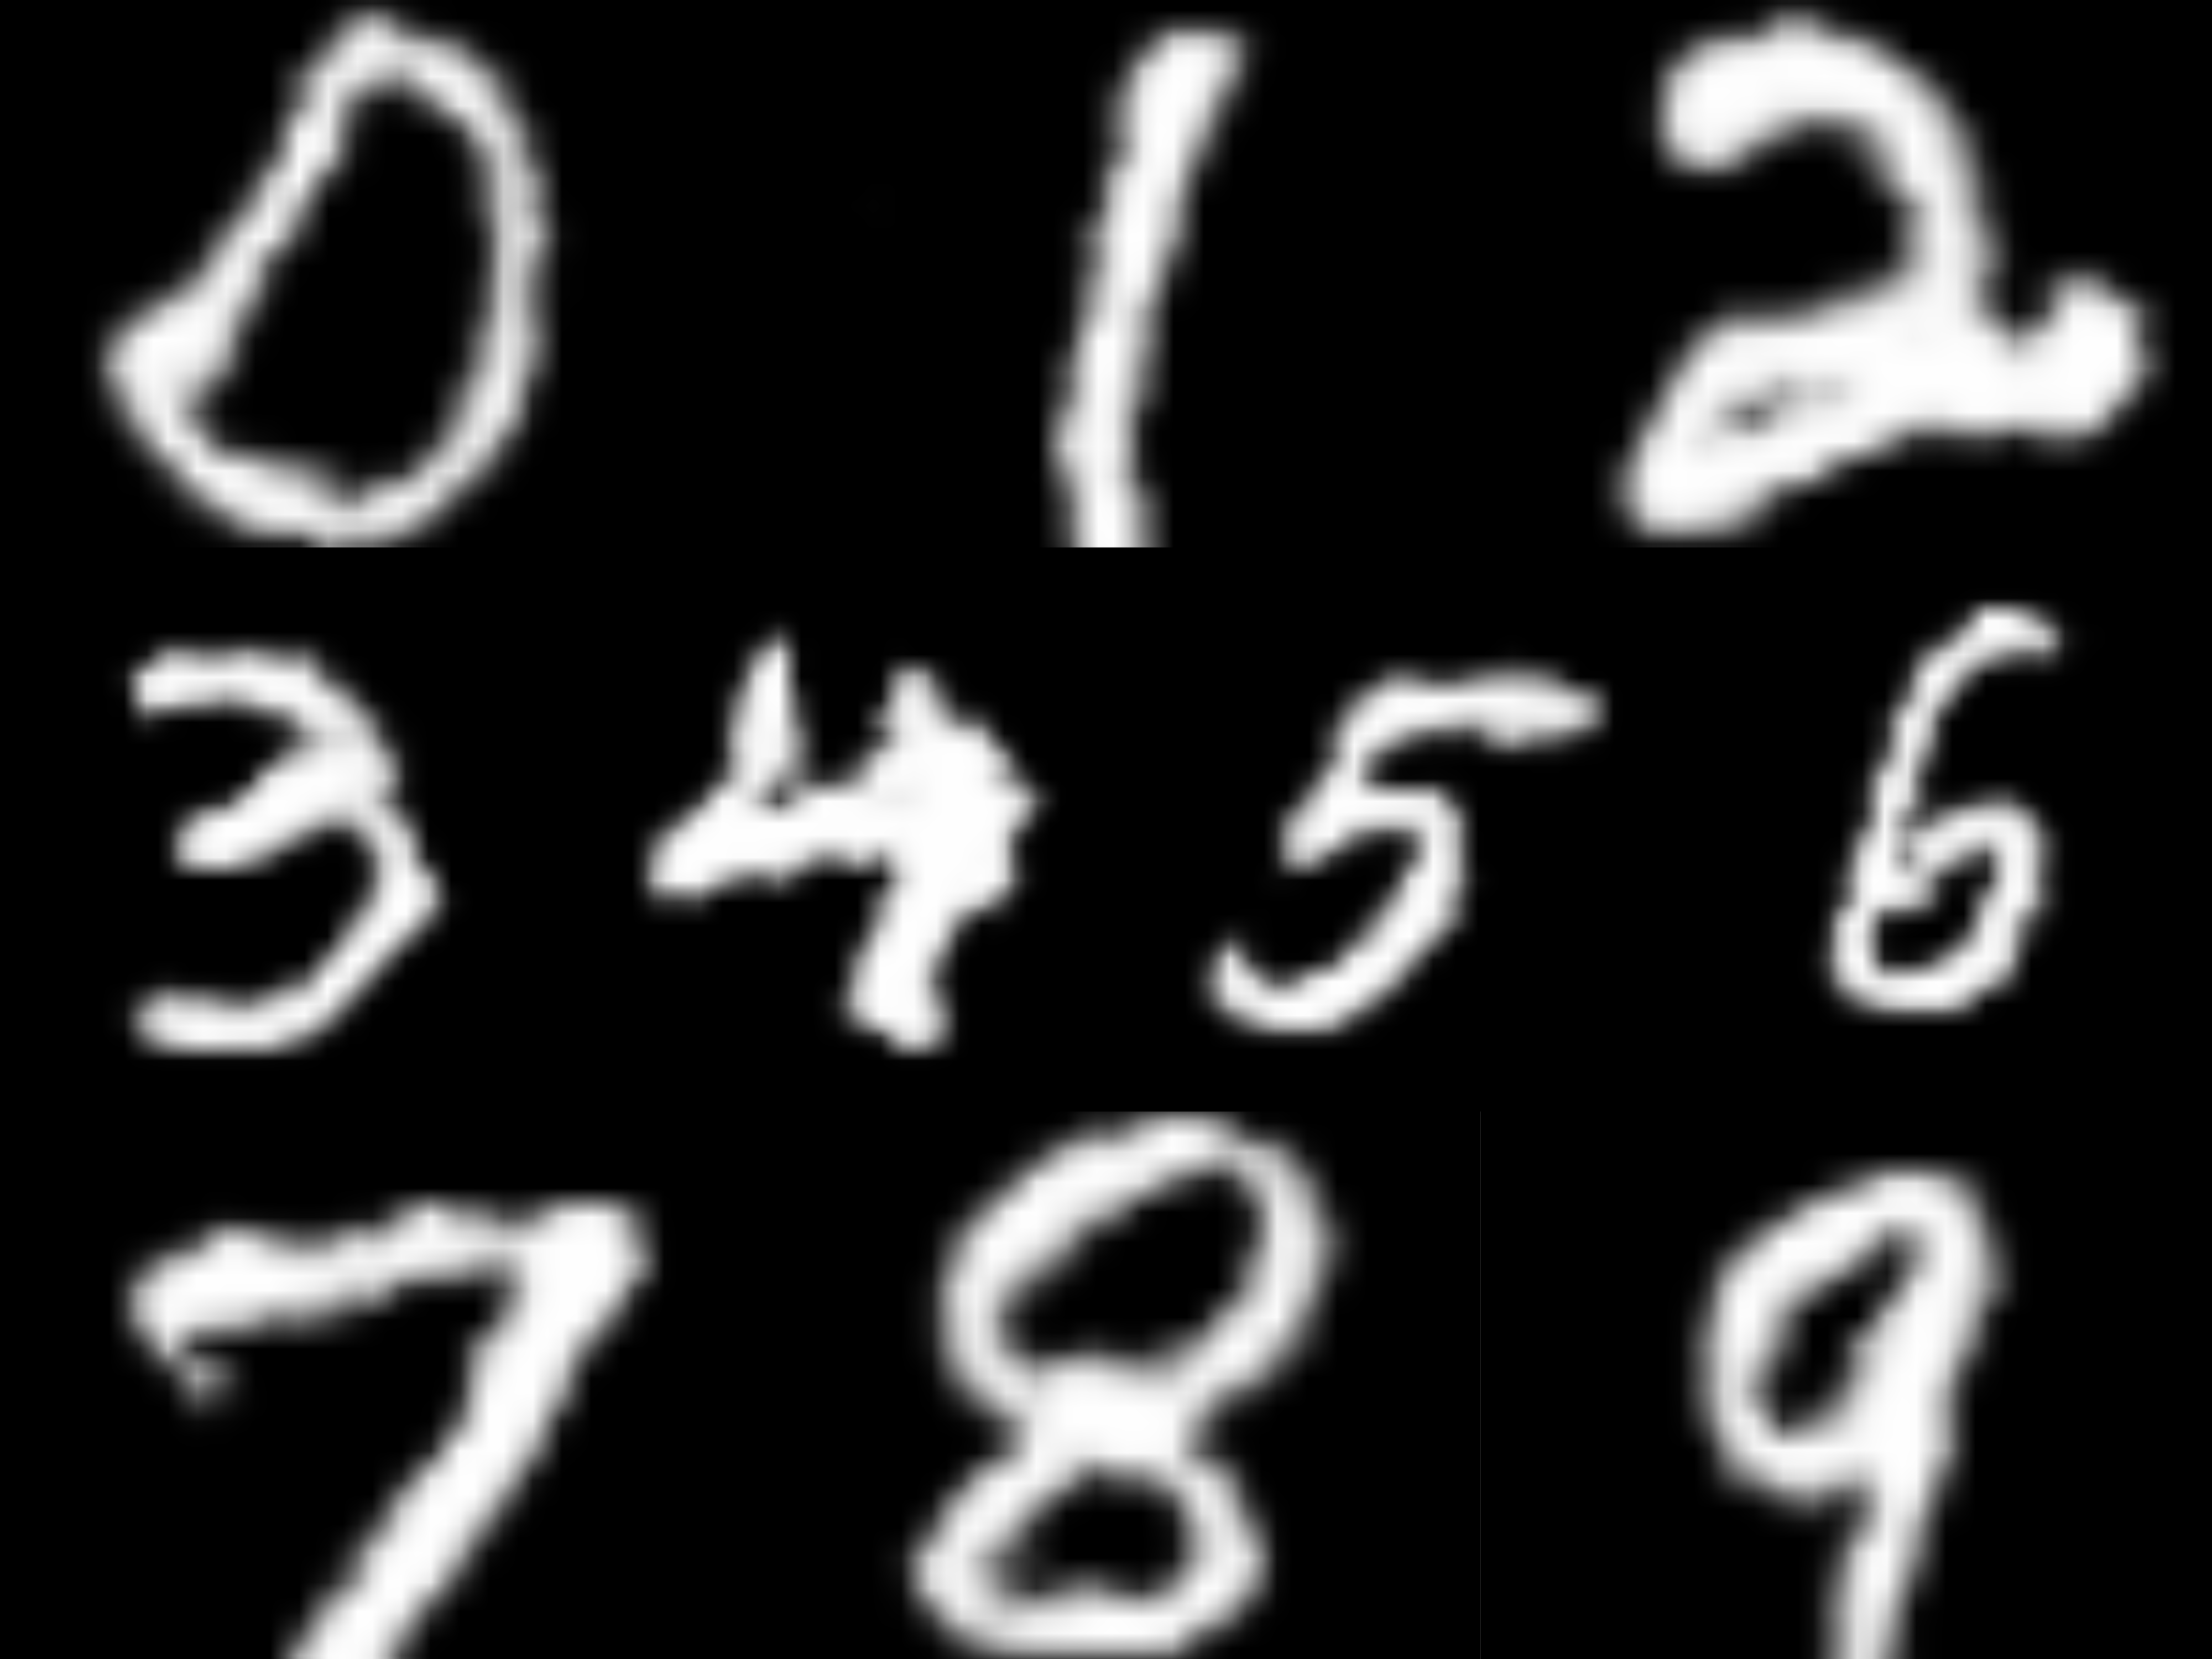
\includegraphics[width=0.4\textwidth]{mnist/resultado_0-9}
\caption{Imágenes generadas con el modelo entrenado con MNIST}
\label{fig:numeros_0-9}
\end{figure}

\subsubsection{Datasets}
El modelo fue entrenado con el dataset COCO en dos variantes. Por un lado, se utilizó el conjunto completo, que ofrece una gran variedad de escenarios y contextos, lo que mejora la generalización del modelo. Sin embargo, su alto requerimiento computacional exigía un entorno potente y tiempos prolongados de entrenamiento.

Por otro lado, se trabajó con subconjuntos aleatorios del dataset, lo que permitía experimentar con mayor agilidad y requerimientos más modestos de memoria. Si bien esto limitaba la generalización, resultó útil para afinar hiperparámetros y realizar pruebas rápidas.

\subsubsection{Pruebas y resultados}
La arquitectura de la cGAN fue adaptada para trabajar con entrada condicionada, lo que implicó modificaciones específicas tanto en el generador como en el discriminador. El generador fue diseñado para recibir un vector de ruido aleatorio concatenado con un vector de características textuales, representando la descripción de la imagen deseada. Este vector conjunto alimentaba una red de capas transpuestas convolucionales que generaban una imagen de salida. Por su parte, el discriminador fue ajustado para aceptar como entrada tanto la imagen generada como la descripción textual correspondiente, evaluando si la imagen no solo era realista, sino también coherente con el texto proporcionado.

Durante el proceso de entrenamiento, se llevaron a cabo múltiples fases de pruebas, con ajustes progresivos que permitieron estudiar el comportamiento del modelo ante diferentes configuraciones:

\begin{itemize}
\item \textbf{Primera etapa:} Se utilizó una tasa de aprendizaje de 0.0002 y se mantuvo una arquitectura básica en el generador y el discriminador. En esta configuración, el modelo logró generar imágenes con formas básicas y contornos generales, pero sin mucho detalle. Las imágenes eran a menudo borrosas y poco realistas, especialmente cuando las descripciones textuales eran más complejas o contenían múltiples objetos.

\item \textbf{Segunda etapa:} Se redujo la tasa de aprendizaje a 0.0001, buscando una mayor estabilidad en el proceso de entrenamiento. Este ajuste permitió al modelo generar imágenes con mayor nitidez en los bordes y una ligera mejora en la estructura general de los objetos. No obstante, aún persistía cierta borrosidad, especialmente cuando el texto incluía relaciones espaciales o adjetivos calificativos que requerían una interpretación semántica más profunda.

\item \textbf{Tercera etapa:} Se realizaron modificaciones más profundas en la arquitectura, incrementando la profundidad de las redes LSTM utilizadas para procesar el texto y añadiendo capas convolucionales adicionales al generador. Estos cambios permitieron al modelo capturar mejor los detalles visuales descritos en las anotaciones textuales. Las imágenes generadas mostraban una mayor fidelidad a las descripciones, especialmente en contextos sencillos o escenas con un número limitado de elementos. Sin embargo, cuando las descripciones eran más complejas, que incluían múltiples objetos en relación o elementos abstractos, el modelo aún presentaba dificultades para generar imágenes coherentes.

\end{itemize}

En conjunto, estas pruebas demostraron que la arquitectura de la cGAN, con un ajuste adecuado de hiperparámetros y arquitectura, era capaz de generar imágenes razonablemente alineadas con descripciones textuales simples, aunque todavía mostraba limitaciones en cuanto a la representación semántica profunda y la calidad visual en escenarios complejos.


\subsubsection{Pruebas con diferentes números de épocas}
Se compararon dos enfoques de entrenamiento para evaluar cuál ofrecía mejores resultados bajo distintas condiciones de entrenamiento y disponibilidad de recursos computacionales:

\begin{itemize}
\item \textbf{Entrenamiento en múltiples fases cortas (menos épocas)}: Este enfoque consistía en entrenar el modelo con un número reducido de épocas, interrumpir el proceso, analizar los resultados obtenidos y realizar ajustes en los hiperparámetros o en la arquitectura antes de retomar el entrenamiento. Su principal ventaja radica en la velocidad de iteración, permitiendo una retroalimentación rápida sobre el comportamiento del modelo. Esto resultó útil especialmente en las primeras fases de desarrollo, donde se requería probar distintas combinaciones de parámetros y realizar modificaciones frecuentes. Sin embargo, se observó que este tipo de entrenamiento limitaba el potencial de aprendizaje del modelo, ya que no se alcanzaban suficientes ciclos de optimización para capturar patrones más complejos del conjunto de datos. Además, las mejoras en la calidad de las imágenes generadas tendían a estancarse tras unas pocas épocas.

\item \textbf{Entrenamiento continuo con muchas épocas}: En contraste, este enfoque implicaba ejecutar el entrenamiento de manera prolongada, permitiendo que el modelo tuviese tiempo suficiente para ajustar de forma más precisa los pesos de sus redes. Esta estrategia fue especialmente efectiva una vez se contaba con una configuración inicial bien afinada, ya que permitía que el modelo convergiera hacia una solución más estable y generara imágenes de mayor calidad. Las imágenes resultantes presentaban mayor nivel de detalle y coherencia con las descripciones textuales. No obstante, este método también conllevaba riesgos, como el sobreajuste, especialmente si los hiperparámetros no estaban correctamente definidos. Además, al requerir mayor tiempo y recursos computacionales, su ejecución resultaba menos viable en fases iniciales de desarrollo o cuando se contaba con recursos limitados.

\end{itemize}

Ambos métodos ofrecieron ventajas complementarias. El entrenamiento en fases cortas fue ideal para la exploración rápida y la experimentación con diferentes configuraciones, mientras que el entrenamiento extendido resultó más adecuado en etapas finales, cuando se buscaba optimizar la calidad del modelo ya ajustado. En el contexto del proyecto, se utilizó una combinación de ambos enfoques: primero se realizaron múltiples entrenamientos breves para afinar la arquitectura y los hiperparámetros, y posteriormente se aplicó un entrenamiento largo con la configuración seleccionada para maximizar el rendimiento final del modelo. Las diferencias entre ambos enfoques, así como sus principales ventajas y desventajas, se resumen en la Tabla~\ref{tab:comparacion_entrenamiento}.


\begin{table}[H]
\centering
\renewcommand{\arraystretch}{1.5}
\begin{tabular}{p{5cm}p{5cm}p{5cm}}
\rowcolor{gray!30}
\textbf{Aspecto} & \textbf{Entrenar varias veces con menos épocas} & \textbf{Entrenar una sola vez con más épocas} \\
\rowcolor{gray!10}
\textbf{Velocidad de iteración} & Alta: permite detectar problemas y ajustar configuraciones rápidamente & Baja: requiere más tiempo para identificar problemas o ajustar parámetros \\
\addlinespace
\textbf{Potencial de aprendizaje} & Limitado, ya que el modelo no alcanza su máximo potencial & Alto, permite que el modelo ajuste mejor los pesos y logre mayor detalle \\
\rowcolor{gray!10}
\textbf{Riesgo de sobreajuste} & Bajo, debido a la menor cantidad de épocas & Alto, especialmente si la configuración inicial no es óptima \\
\addlinespace
\textbf{Calidad de las imágenes} & Adecuada para configuraciones iniciales, pero se estanca en calidad final & Mejor calidad, con imágenes más detalladas y coherentes \\
\rowcolor{gray!10}
\textbf{Flexibilidad en ajustes} & Alta: permite ajustar configuraciones con mayor frecuencia & Baja: los errores solo se detectan al final del proceso \\
\addlinespace
\textbf{Uso de recursos} & Menor uso de recursos en cada iteración & Mayor uso de recursos debido a entrenamientos más largos \\
\rowcolor{gray!10}
\textbf{Idoneidad} & Ideal para experimentación y ajustes rápidos & Adecuado para optimización final con configuraciones ajustadas \\
\end{tabular}
\caption{Comparativa entre entrenar con menos épocas y entrenar con más épocas}
\label{tab:comparacion_entrenamiento}
\end{table}

\subsubsection{Visualización de pérdidas}
Las curvas de pérdida registradas durante el entrenamiento (Figura~\ref{fig:loss_curve_cgan}) muestran que el discriminador aprende rápidamente en las primeras épocas, con una pérdida que disminuye de forma pronunciada. En contraste, el generador progresa más lentamente, con una pérdida que decrece gradualmente. Este comportamiento es común en las cGAN, y si no se controla, puede llevar a un desequilibrio en el entrenamiento. En este caso, el discriminador tendía a dominar, lo que podría afectar negativamente la calidad de las imágenes generadas.

\begin{figure}[H]
\centering
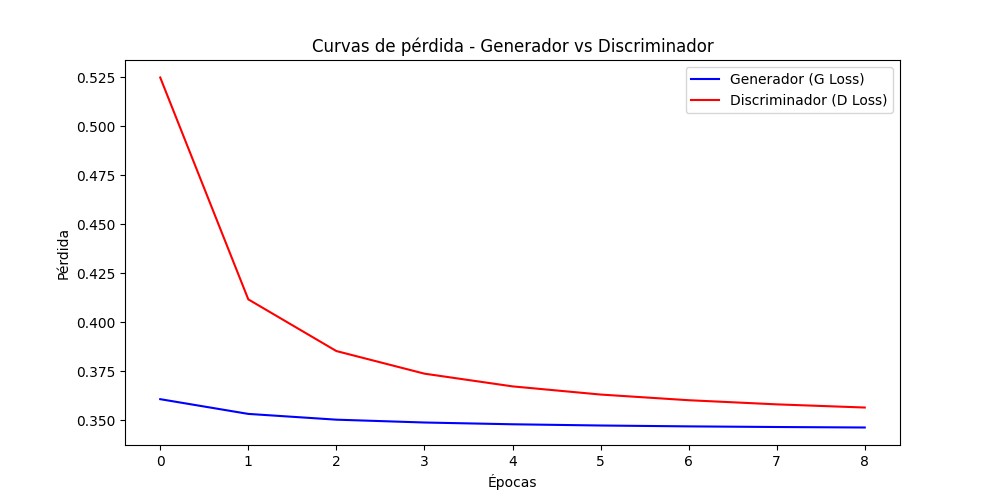
\includegraphics[width=0.7\textwidth]{perdidas}
\caption{Curva de pérdidas durante el entrenamiento de la cGAN}
\label{fig:loss_curve_cgan}
\end{figure}

\subsubsection{Conclusión}
La cGAN permitió integrar las descripciones textuales en el proceso de generación de imágenes, obteniendo mejores resultados que con la GAN básica. Sin embargo, el modelo mostró dificultades para representar con nitidez descripciones complejas. Esto motivó la exploración de modelos más sofisticados como la AttnGAN, que incorpora mecanismos de atención para mejorar la correspondencia entre texto e imagen.

\subsection{Atención textual: AttnGAN}
AttnGAN representa una evolución respecto a la cGAN, especialmente en cuanto a estabilidad durante el entrenamiento y eficiencia en la gestión de recursos computacionales. A diferencia de las cGANs implementadas en TensorFlow, AttnGAN se desarrolló sobre PyTorch, lo que permitió un mayor control sobre la asignación de memoria y una mejor capacidad para manejar grandes volúmenes de datos. Este modelo está específicamente diseñado para generar imágenes a partir de descripciones textuales mediante el uso de mecanismos de atención, que permiten asociar palabras o fragmentos específicos del texto con regiones concretas de la imagen. Este enfoque favorece una mayor coherencia semántica entre el contenido textual y visual, y mejora el nivel de detalle generado en las imágenes.

\subsubsection{Configuración del entrenamiento}
El modelo fue entrenado utilizando el dataset COCO completo, el cual proporciona una gran variedad de imágenes junto con múltiples descripciones por imagen, lo que resulta ideal para tareas de generación condicionada por texto. Gracias a la eficiencia de PyTorch en la gestión de memoria, no fue necesario trabajar con subconjuntos del dataset, como sí ocurrió en el caso de la cGAN. El entrenamiento se realizó en la plataforma Kaggle, que ofrece acceso gratuito a GPU pero impone una limitación de 30 horas semanales de ejecución. Esta restricción obligó a limitar el entrenamiento a un máximo de 40 épocas por ejecución completa.

A pesar de esta limitación temporal, la estabilidad del entrenamiento fue notable. PyTorch permitió mantener un tamaño de batch razonable sin generar errores de memoria, lo que favoreció una convergencia progresiva y consistente. Asimismo, el modelo integra mecanismos de atención en múltiples niveles: en cada etapa del proceso generativo, el sistema aprende a enfocar su atención en las partes más relevantes de la descripción textual, optimizando así la correspondencia entre texto e imagen.

\subsubsection{Proceso de entrenamiento}
El entrenamiento de AttnGAN se dividió en varias fases, cada una diseñada para evaluar y refinar la calidad de las imágenes generadas. Aunque el límite de 40 épocas restringía el alcance del entrenamiento, fue posible observar una mejora progresiva en la correspondencia entre texto e imagen. En comparación con la cGAN, donde la pérdida era altamente inestable, AttnGAN mostró una evolución más suave y coherente, aunque no se generaron curvas de pérdida formales para su análisis.

En ausencia de métricas cuantitativas detalladas, se utilizó una estrategia de evaluación visual para examinar las imágenes generadas a lo largo del entrenamiento. Esta evaluación permitió ajustar los hiperparámetros, como la tasa de aprendizaje y la arquitectura de las capas intermedias, en función de la calidad perceptual observada. En futuras implementaciones, contar con un sistema de logging más completo permitiría extraer información cuantitativa útil para complementar esta evaluación.

\subsubsection{Resultados y evaluación visual}

A nivel de resultados, AttnGAN logró generar imágenes que reflejaban de forma razonable la estructura y los elementos clave descritos en el texto. En particular, se utilizó como entrada el prompt \textit{``A man with a red jacket riding a motorcycle in the woods''}, que describe una escena compleja con múltiples objetos y relaciones espaciales. La imagen generada, mostrada en la Figura~\ref{fig:attn}, transmite adecuadamente la intención general del texto: puede apreciarse una figura central clara, asociada al conductor y su motocicleta, rodeada de un entorno con colores verdes y marrones que sugiere vegetación.

No obstante, las imágenes seguían presentando borrosidad y falta de precisión en los detalles, lo que limitaba su aplicabilidad en contextos que requieran imágenes de alta fidelidad.

\begin{figure}[H]
\centering
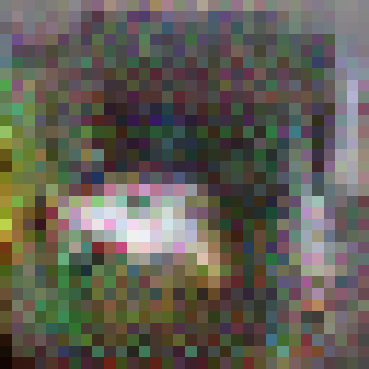
\includegraphics[width=0.4\textwidth]{generated_image_epoch_10}
\caption{Mejor imagen generada por AttnGAN durante el entrenamiento con el prompt: \textit{``A man with a red jacket riding a motorcycle in the woods''}}
\label{fig:attn}
\end{figure}

\subsection{Modelo final}
Tras varias iteraciones exploratorias con distintos modelos generativos desarrollados desde cero, se optó finalmente por utilizar un modelo preentrenado que resolviera las limitaciones encontradas en cuanto a recursos y calidad de imagen: \textit{Stable Diffusion v1.4}.

\subsubsection{Motivación para el uso de modelos preentrenados}
A lo largo del proyecto, se implementaron modelos como GAN, cGAN y AttnGAN. Estas aproximaciones permitieron comprender la lógica interna de la generación de imágenes, así como los desafíos vinculados a la representación del texto y la arquitectura del generador. Sin embargo, la calidad de las imágenes generadas no era suficiente, y el coste computacional resultó demasiado elevado. Por ello, se decidió adoptar un modelo preentrenado robusto como Stable Diffusion, que ofreciera resultados inmediatos y una mayor fidelidad visual.

\subsubsection{Descripción del modelo}
Stable Diffusion es un modelo generativo basado en la técnica de difusión latente. Su funcionamiento se basa en partir de una imagen compuesta únicamente por ruido, que se refina progresivamente gracias a una red neuronal convolucional condicionada por el texto de entrada.

\subsubsection{Componentes principales}
\begin{itemize}
    \item \textbf{UNet:} red neuronal convolucional encargada del proceso de denoising, refinando la imagen en cada paso de inferencia.
    \item \textbf{Text Encoder (CLIP):} transforma la descripción textual en un espacio latente de características que orienta el proceso de generación.
    \item \textbf{Autoencoder Variacional (VAE):} codifica las imágenes reales y decodifica los resultados generados en un espacio latente comprimido.
    \item \textbf{Scheduler:} controla el nivel de ruido introducido en cada iteración de difusión, determinando la evolución temporal del proceso.
\end{itemize}

\subsubsection{Parámetros del modelo}
\begin{itemize}
    \item Resolución de entrada: \textbf{512x512 píxeles}.
    \item Pasos de inferencia: \textbf{50}.
    \item Escala de orientación: \textbf{7.5} (Guidance Scale).
    \item Tamaño del espacio latente: \textbf{64x64 píxeles}.
    \item Codificador de texto: \textbf{CLIP ViT-L/14}.
    \item Tamaño del modelo UNet: aproximadamente \textbf{860M de parámetros}.
\end{itemize}

\subsubsection{Prueba inicial de generación}
Como primer experimento de validación, se utilizó el prompt:

\begin{center}
\textit{``A beautiful landscape with mountains and a river''}
\end{center}

Se emplearon los valores por defecto del modelo y se obtuvo la siguiente imagen:

\begin{figure}[H]
    \centering
    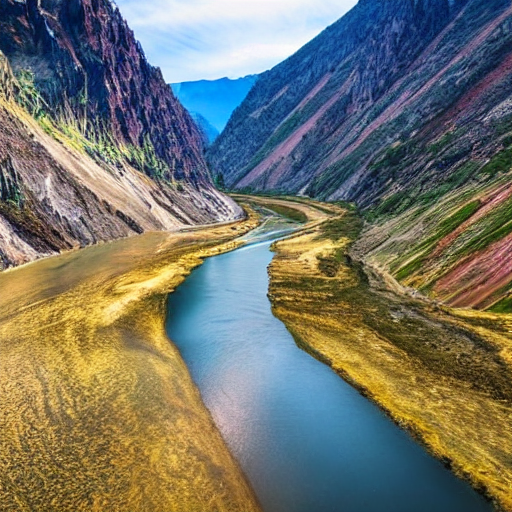
\includegraphics[width=0.4\textwidth]{original_output_image.png}
    \caption{Imagen generada con Stable Diffusion v1.4}
    \label{fig:original_image}
\end{figure}

\subsubsection{Conclusiones preliminares}
La prueba demostró que Stable Diffusion proporciona imágenes de gran calidad visual con una alta coherencia respecto a la descripción textual. Su uso supuso una mejora inmediata en términos de rendimiento y viabilidad para su integración con la plataforma Java.

\subsubsection{Optimización del modelo}
Aunque el modelo preentrenado ya ofrecía resultados prometedores, se exploraron posibles optimizaciones para mejorar aún más la precisión y adaptabilidad del sistema:

\begin{itemize}
    \item \textbf{Ajuste fino del modelo completo:} consiste en reentrenar el modelo en su totalidad utilizando un nuevo conjunto de datos, lo que permite adaptar todos sus parámetros a una tarea específica. Esta técnica mejora la especialización del modelo, aunque requiere muchos recursos computacionales y riesgo de sobreajuste si no se dispone de suficientes datos.

    \item \textbf{Modificación del espacio latente:} se centra en ajustar la estructura o dimensiones del espacio latente donde se representan las imágenes. Esto puede permitir una mayor expresividad y detalle en las imágenes generadas, así como un mejor alineamiento semántico entre el texto y la imagen.

    \item \textbf{Sustitución del decodificador VAE:} implica reemplazar el decodificador del autoencoder variacional por otro más potente o con características distintas, con el objetivo de mejorar la calidad visual de las imágenes reconstruidas desde el espacio latente.

    \item \textbf{Entrenamiento LoRA (Low-Rank Adaptation):} permite ajustar solo un pequeño subconjunto de parámetros del modelo base de forma eficiente, reduciendo el coste computacional y el riesgo de sobreajuste. Es especialmente útil cuando se quiere adaptar el modelo con recursos limitados.

    \item \textbf{Cambio en funciones de pérdida:} implica modificar la función de coste que guía el aprendizaje del modelo. Por ejemplo, se puede incorporar una pérdida perceptual o una pérdida basada en CLIP para mejorar la coherencia semántica entre la imagen y el texto.

    \item \textbf{Adaptaciones en la arquitectura UNet:} consiste en modificar la red UNet responsable del proceso de denoising durante la difusión. Esto puede incluir la incorporación de capas de atención adicionales, cambios en la profundidad de la red o en su estructura de skip connections para mejorar la capacidad del modelo.
\end{itemize}

\subsubsection{Optimización seleccionada: modificación del espacio latente}
Entre todas las alternativas exploradas, se optó por modificar el espacio latente del modelo mediante un proceso de ajuste personalizado inspirado en la técnica DreamBooth. En lugar de utilizar herramientas empaquetadas, se implementó un procedimiento propio en Python que permite especializar el modelo de difusión en nuevas clases visuales, partiendo de una colección reducida de imágenes.

Para ello, se seleccionaron 60 imágenes de tres razas concretas de perro (\textit{golden retriever}, \textit{basset hound} y \textit{whippet}) del dataset Stanford Dogs. Estas imágenes fueron preprocesadas y utilizadas en un entrenamiento supervisado en el que:

\begin{itemize}
    \item Se congelaron los módulos del codificador de texto (\texttt{CLIPTextModel}) y el decodificador (\texttt{AutoencoderKL}).
    \item Se entrenó únicamente la red \texttt{UNet2DConditionModel}, que controla la predicción del ruido en el espacio latente.
    \item Se empleó un prompt específico (\texttt{a photo of a sks dog}) como condicionamiento textual, simulando la incorporación de una nueva categoría visual.
\end{itemize}

Este entrenamiento se realizó con un tamaño de lote de 1, utilizando el optimizador AdamW y una tasa de aprendizaje reducida (\texttt{5e-6}), durante 1000 pasos. Una vez completado el entrenamiento, se generaron imágenes de prueba con prompts específicos para cada raza, como \texttt{``a photo of a sks whippet wearing sunglasses''}.

\begin{itemize}
    \item Se observó un aumento en la nitidez y realismo de las imágenes generadas.
    \item Las imágenes eran coherentes con los conceptos entrenados y semánticamente alineadas con los prompts.
    \item El coste computacional fue contenido al reutilizar componentes preentrenados y entrenar únicamente los parámetros necesarios.
\end{itemize}

Este enfoque proporciona un equilibrio óptimo entre rendimiento, especialización visual y eficiencia, y resulta especialmente útil para entornos integrados como JMR.

\begin{figure}[H]
    \centering
    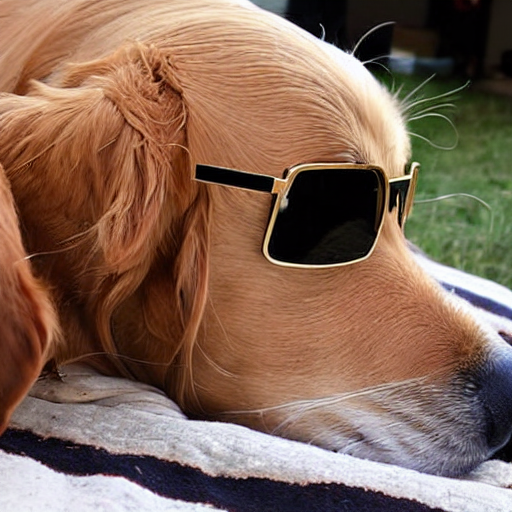
\includegraphics[width=0.45\textwidth]{golden retriever.png}
    \hfill
    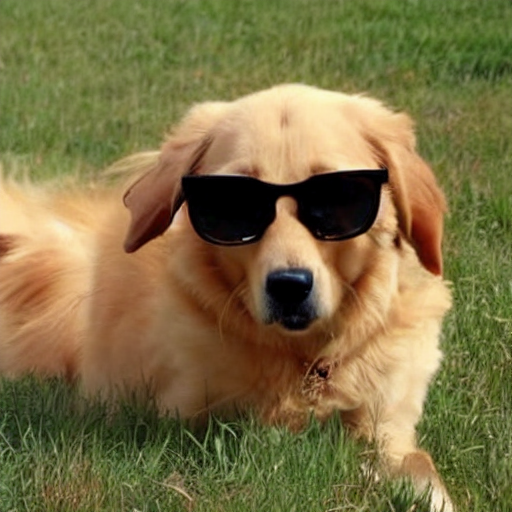
\includegraphics[width=0.45\textwidth]{golden retriever-2.png}
    \caption{Ejemplo de imágenes generadas tras la modificación del espacio latente}
    \label{fig:latent-space-optimization}
\end{figure}